

\section{Supporting Data Environments with W3C PROV} \label{sec:impl}
The W3C PROV data model structure and elements supports some of the data environment representation requirements. Because the elements of data environments can be mapped with PROV elements. PROV  properties can be used to represent the semantic relationship among the elements of data environment. However, there are some data environment specific requirements  that need extensions in PROV. In the following sub-sections we will explain how PROV can be applied to support data environment representation through four possible mechanisms.

\subsection{PROV Bundle}
In PROV, the bundle concept has some similarities to the data environment construct. %\todo{[ref]} \todo[color=green!40]{I didn't found any suitable reference. But from the explanation it is visible that they created bundle for similar purpose such as to capture provenance in multiple environments, so they can stitch it together. we can also remove this line if PROV baby looks ugly!\dSmiley}. 
The bundle itself is an entity which provides the provenance information of creation and modification of group of entities \cite{mckenna2019modelling}. 
%A bundle can also hold the provenance of other elements. 
For example a bundle can contain the entities, activities, agents, and the relationships between them. %This would enable us to represent the data controller, data processor, data subjects, and data users with the  \textit{PROV agent construct}. 
The  data, and data processes can be expressed with entities, and activities respectively. Bundles can also support entities with attributes. This can help us to add necessary metadata to the entities. 
%For example, essential means of data collection of GOND-NRDS use case can be expressed with additional metadata attachment to the entities inside the bundles. 
The excerpt view of the GOND-NRDS use case representation as supported by PROV bundles is shown in Figure \ref {fig:bundle}.

\begin{figure}[!htbp]
%\centering
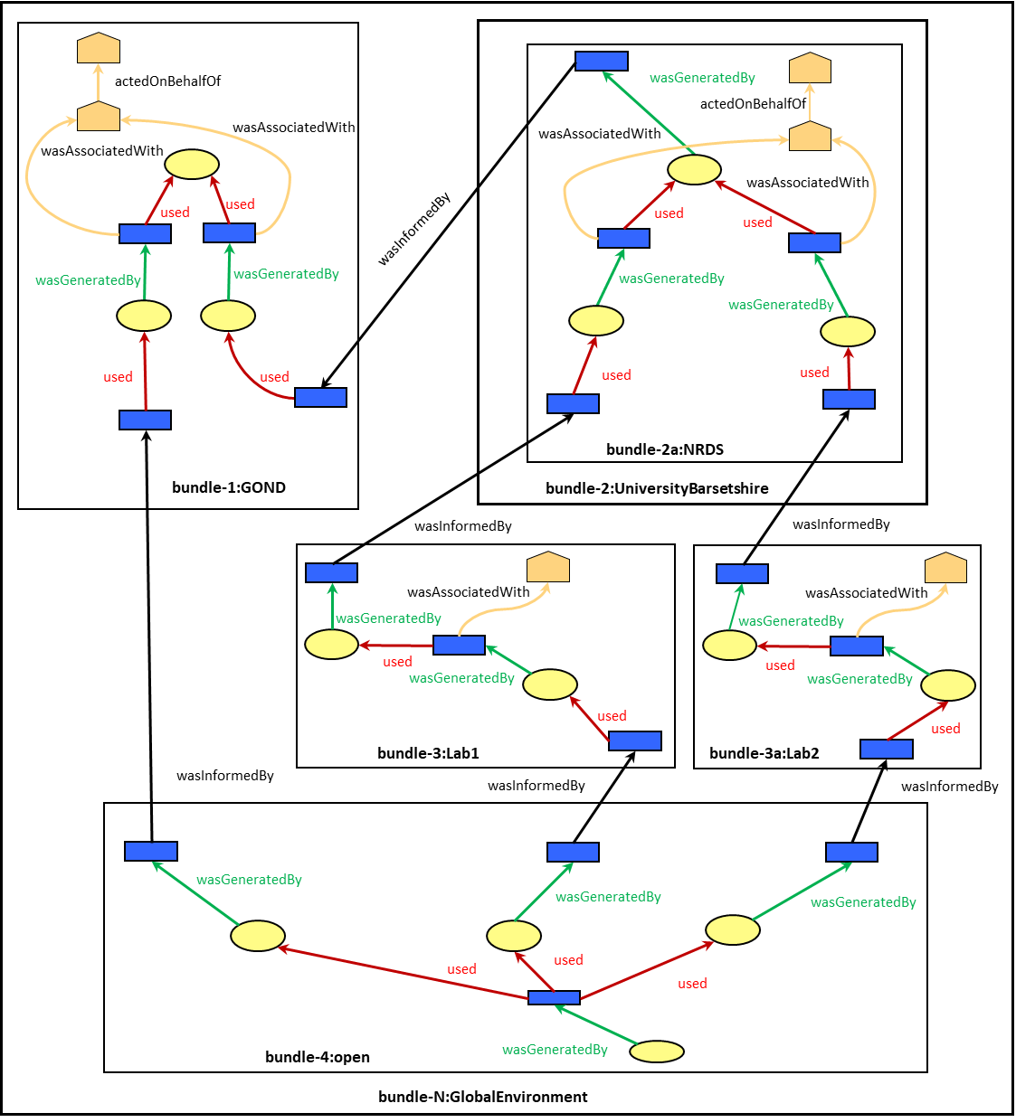
\includegraphics[width=\linewidth, height=8cm]{bundle.png}
\caption{A representation of the GOND-NRDS use case supported with PROV bundles} \label{fig:bundle}
\end{figure}

\subsection{Namespaces} \label{subsec:namespaces}
Namespaces are a Uniform Resource Identifier (URI). A provenance graph can contain many Namespaces. In PRVO-DM, the Namespace concept was inspired by the World Wide Web architecture and was designed to make objects interoperable across technologies and platforms \cite{moreau2015rationale}. 
PROV Namespace is a candidate for use as an identifier to capture the idea of multiple data environments (including data environments within data environments) and their associated entities, activities, agents, etc. 
By using Namespaces and  prefixes we can differentiate the representation of nested data environments and  can access related elements information through Namespace concatenating and de-concatenating. For example, we can refer the data environment of University  Baretshire and NRDS data environment (Note: In the use case NRDS data environment is a part of University Baretshire environment) as \textit{http://global-env.com/bu/ 
} and  \textit{http://global-env.com/bu/nrds/ 
} respectively. Additionally, we can also express the control mechanism over the data environments and its elements  with  Namespace feature. The visual representation of the GOND-NRDS use case  with the support of Namespaces and PROV constructs is shown in Figure \ref{fig:namespaces}.


\subsection{Namespaces with Support Structures} \label{subsec:namespacesplus}
While namespaces are powerful with respect to representing data environments boundaries, and what has occurred within a given data environment, and it's sub-data environments, namespaces themselves are not enough to satisfy all of the requirements identified within the use case. For instance, the attachment of additional attributes to the Data Environment itself and contracts between the data environments  cannot be accommodated. Additionally, relationships among namespaces beyond containment cannot be captured. For instance, it is possible with namespaces to distinguish that \textit{ http://www.nytimes.com}  data environment that contains a sub-data environments related to advertising functions, \textit{http://www.nytimes.com/ads}. However, within our use case, there is more than strict-hierarchical containment. On occasion, researchers from Research Labs have a specialized data analysis environment built-by, hosted-by and managed-by NRDS, but is considered an enclave of both NRDS and the Research Lab. In this case, namespaces do not capture enough information to represent this relationship.

To solve this, an additional set of structures would need to be created. For instance, a separate document which extends namespaces and allows attachment of attributes, could be utilized. 

\begin{figure}[!htbp]
%\centering
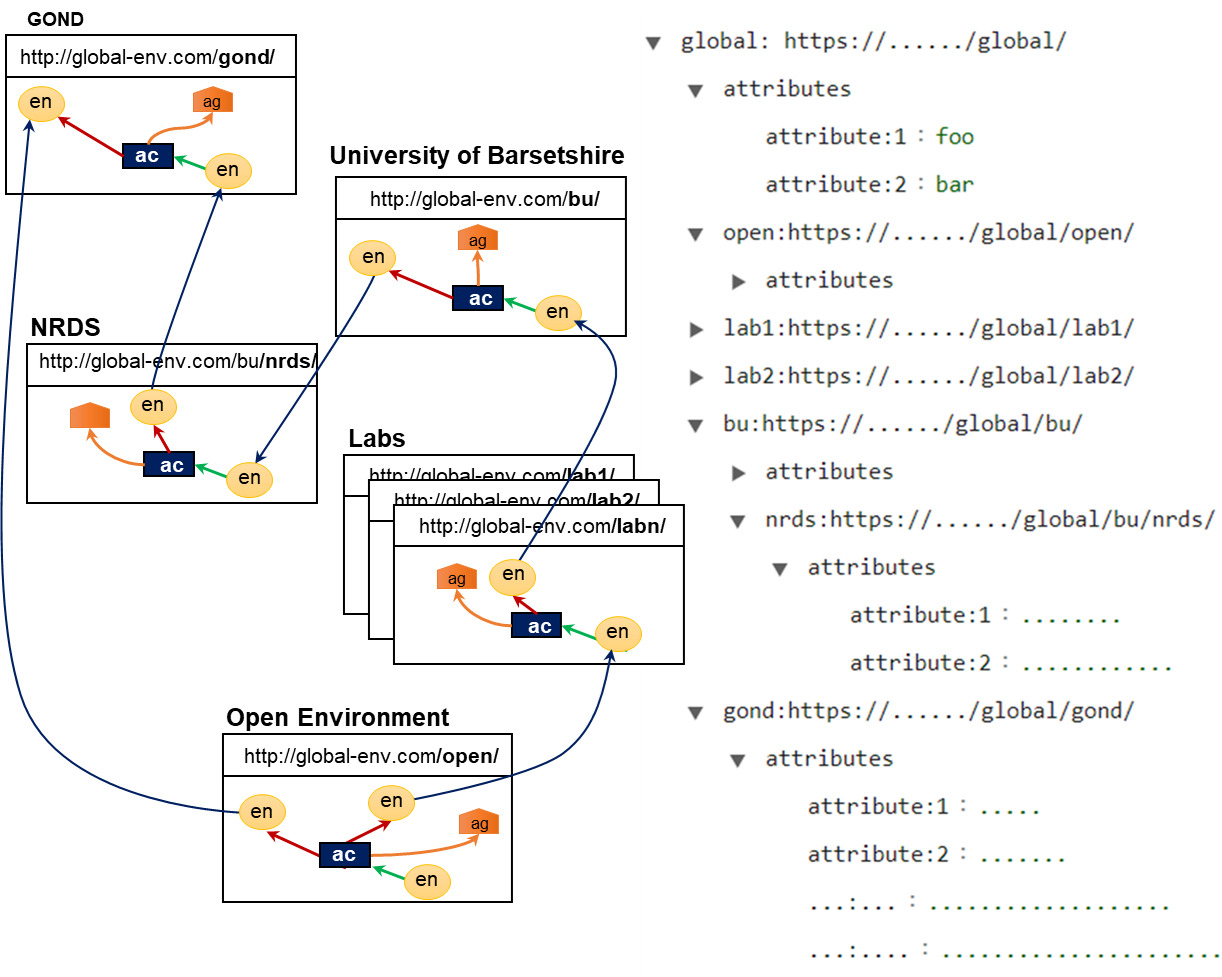
\includegraphics[width=\textwidth]{namespaces-2.png}
\caption{Illustration of the use of Namespaces to represent Data Environments: ag, ac, and en indicates agent, activity, and entity respectively; the right hand part  shows data environments with attribute attachment using Namespaces. Relationships across namespaces could be captured in the same manner. } \label{fig:namespaces}
\end{figure}

\subsection{Extended Bundles}   

W3C PROV constructs\footnote{The constructs are  structure and elements that are used to express the provenance of any object or thing.} were designed to be extensible \cite{moreau2015rationale}. PROV has already been extended to express the provenance of Big data security supervision \cite{gao2020big}, provenance access control \cite{missier2020abstracting}, data privacy protection based on GDPR using provenance \cite{davari2019access} and  managing mutable entities by adding reference derivations and checkpoints \cite{pimentel2018versioned}.
Similarly, we can extend the existing structure of PROV bundles in order to support and express the requirements of ADF  with better flexibility. For example, by extending we can attach  additional metadata with the bundle construct, which is necessary to define the types of  GOND-NRDS data environments. Another extension that we might need in PROV Bundles, is to support  nested data environments. if we consider the PROV bundle as a named set for the representation of data environment. On the other hand we can extend PROV by adding the new component (e.g. \textit{dataEnvironment}, \textit{endDataEnvironment}) for the data environment as a first class candidate and develop a new layer over the bundle structure. As a second step we could then build a mechanism to include attributes, entities, activities, agents, etc in each \textit{dataEnvironment}. In this approach, we can also reuse some of the existing features of bundles and entities. 

%comment by Age
\begin{comment}
Hang on here. Are there actually 2 things in this? 1) extend bundles and 2) make a new thing called data environments? If so, then we actually have 4 possible implementation strategies, and we need a new subsection to split them out (and analysis in that section, etc.  

However, I think what we actually have is a way to create data environments as first class citizens - by extending bundles. 

Could you comment on which it is?
\end{comment}

%comment by aslam
\begin{comment}
Actually this subsection previous title was "How PROV can be extended to support data environment" 

 possibly there are  three ways: 1) updated the bundle mechanism, 2) add data environment as a first class citizen

3) Namespaces with extra support of resources and documents as you described in paragraph starting with however... in section 3.2.  But I wondered  PROV community does not described Namespace likely Bundle, entity, etc. 

4.??? 
 can we leave this or for another paper?
\end{comment}
\begin{comment}
The first option might not be a suitable due to the nested data environments requirement. Because bundle neither supports bundle in a bundle and nor it provides the functionality of attributes attachment with the data environments. Therefore, the second option might take extra efforts but it will enables the comprehensive representation of data environments features. The requirement of similar  entities in multiple data environments  is relatively is a modelling and validation issue. This can be resolved as: 
\begin{itemize}
\item Like in object-oriented programming a variable with the same name can be declared in the class and multiple methods. However, the scope of the variable is limited to the class and methods in which it was declared. 
\item Similarly, there should be the support of multiple similar entities in multiple data environments within the same PROV document. And their scope should be limited to the data environment in which it is declared without explicitly indicating with prefixes.    
\end{itemize}

To resolve the issue of semantic annotation to properties two approaches can be possible. The first option is to  change non-semantic linking properties concepts and tags in the data model and change the labels for properties based on the application domain. The second option is to extend the mechanism of existing properties and introduce the "annotation to property" concept. We think that that the first option needs a continuous changes in the conceptual model and provenance document validation process because the properties concept and naming needs to be updated based on the use case. The second approach is suitable in the case of   data environment representation. Because all the existing properties and validation mechanism will be same, only the annotation attribute value will be updated based in the context of use case.
\end{comment}
